\begin{homeworkProblem}[16][Graph for 16(f)]
Basically this model seems to be one variation of \textbf{S}usceptible 
\textbf{I}nfected \textbf{R}ecovered model (referenced to the {\color{blue} https://plus.maths.org/content/mathematics-diseases}).
I assume that it will result in oscillation of cases: something 
that might look like this:
\begin{figure}[htbp]
    \centering
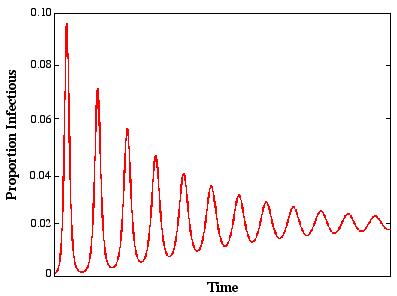
\includegraphics[scale=0.6]{fig/fig(16)(suppose).png}
\caption{Credit to {\color{blue} this website: https://plus.maths.org/content/mathematics-diseases}}
\end{figure}

However, I can only plot figures like this:
\begin{figure}[htbp]
    \begin{subfigure}{0.4\linewidth}
    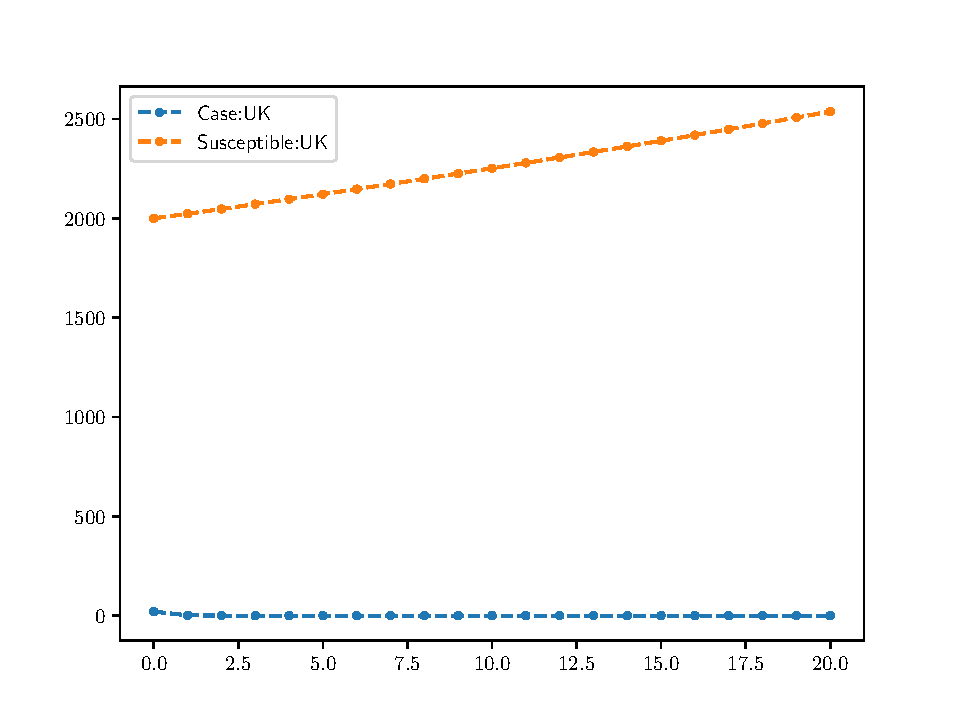
\includegraphics[scale=0.6]{fig/fig16(f)(1).pdf}
    \caption{Model using statistics for UK}
    \end{subfigure}
    \hfill
    \begin{subfigure}{0.4\linewidth}
    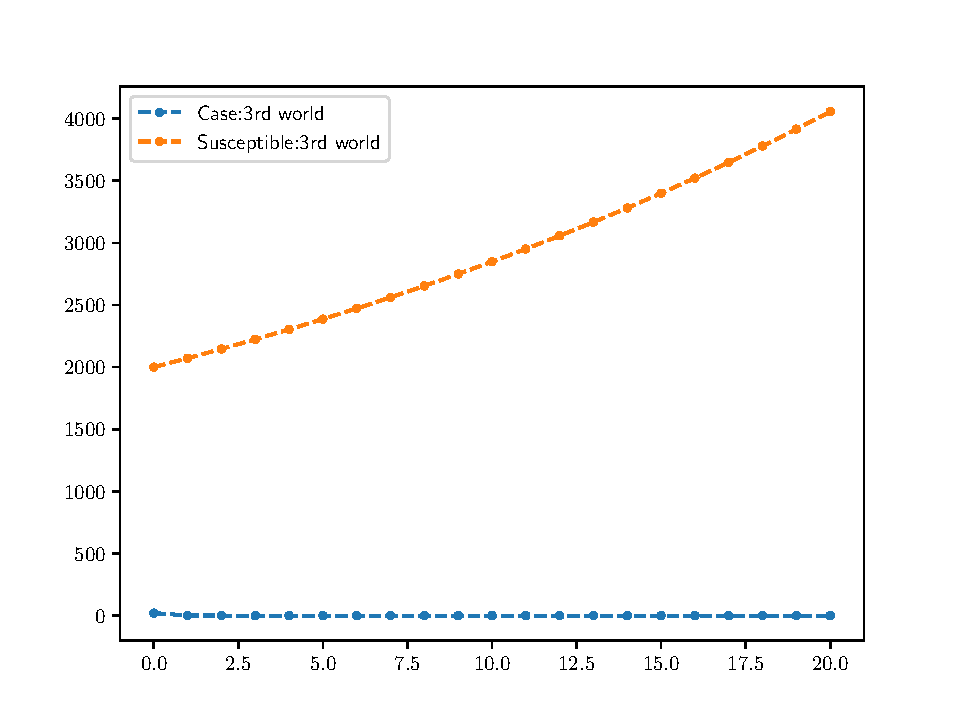
\includegraphics[scale=0.6]{fig/fig16(f)(2).pdf}
    \caption{Model using statistics for 3rd world}
    \end{subfigure}
    \caption{Graphs for 16(f) but not as expected}
\end{figure}


\end{homeworkProblem}